\documentclass[11pt]{article}

% parameters are fairly self-explanatory here, thankfully
\usepackage[width=7in,height=9.5in,top=0.75in,centering]{geometry}

% for math-ing
\usepackage{amsmath}
\usepackage{amssymb}
\usepackage{comment}

%%%%%% tables %%%%%%%%
\usepackage{tabularx}
\usepackage{array}
\renewcommand{\arraystretch}{1.5}
\setlength{\tabcolsep}{8pt}

%%%%%% plotting %%%%%%

\usepackage[dvipsnames]{xcolor}
\usepackage{tikz}
\usepackage{pgfplots}

\pgfplotsset{every axis/.append style={
                    axis x line=middle,    % put the x axis in the middle
                    axis y line=middle,    % put the y axis in the middle
                    axis line style={<->,color=black}, % arrows on the axis
                    xlabel={$x$},          % default put x on x-axis
                    ylabel={$y$},          % default put y on y-axis
            }}
            
 \pgfplotsset{compat=1.14} % sometimes, everything falls apart without this
 
 %\usepgfplotslibrary{fillbetween} %for shading between curves

%%%%%% commands %%%%%%

% exam heading; course name is first argument, exam information is second argument
\newcommand{\Heading}[2]{
    \fbox{
        {\Large\textbf{#1}}
        }
    \hfill
    \fbox{
        \begin{minipage}{0.2\textwidth}
            \begin{center}
            \textbf{#2}
            \end{center}
        \end{minipage}
    }
    \par\vspace{0.1in}}

% for being lazy while beautifying integrals
\newcommand{\dint}{\displaystyle\int}

% for being lazy while beautifying limits
\newcommand{\dlim}{\displaystyle\lim}

%%%%%% stuff %%%%%%

\usepackage{fancyhdr}

%\setcounter{page}{0} % first page is page 0

\parindent0pt % no indent

\fboxsep=0.25cm % little space in fbox border

%%%%%% BEGIN! %%%%%%%

\begin{document}

\pagestyle{fancy}

% record goals here to create sense of transparency

\fancyhead[c]{%
  \ifcase\value{page}
    \or {}
    \or {}
    \or {}
  % empty test for page = 0
  % \or {}% 
  % \or
  \or {\bf\color{ForestGreen} FE1(D1): Meaning of a Derivative}% page=1
\or {\bf\color{ForestGreen} FE2(D2): Compute Derivatives}% page = 3
  \or {\bf\color{ForestGreen} FE3(D3): Derivatives of Basic Functions}% page = 2
  \or {\bf\color{Fuchsia} FE4(I1): Meaning of an Integral}% page = 4
  \or {\bf\color{Fuchsia} FE5(I3): Antiderivatives and Indefinite Integrals}% page = 5
  \or {\bf\color{Fuchsia} FE6(I4): Compute Definite Integrals}% page = 6
  \or {\bf\color{ProcessBlue} FE7(F3): Summations}% page = 7
  \or {\bf\color{RoyalBlue} FE8(L1): Limits and Continuity}% page = 8
  \or {\bf\color{Orange} FE9(P1): Discrete Random Variables}
  \or {\bf\color{Orange} FE10(P2): Continuous Random Variables}
  \else
  % Empty chead here!
  \fi
}

\thispagestyle{empty} % don't display that this is page 0

\Heading{MATH 1190/1210 Survey of Calculus I}{Final Exam Part 1: FE Targets\\Spring 2026}

\vspace{0.1in}

\textbf{Name} \hrulefill \, \begin{minipage}{0.16\textwidth}\begin{center}\textbf{UVA ID\\ (e.g. hdj4nd)} \end{center}\end{minipage}\hrulefill\\

\begin{minipage}{0.2\textwidth}\begin{center}\textbf{Course \&\\ Section Number} \end{center}\end{minipage} \hrulefill\,\,\textbf{Date} \hrulefill  \\

\hrulefill
\paragraph*{Course \& Section Numbers:}

{\small
\begin{center}
\begin{tabular}{| c | c | c | c |}
\hline
\begin{minipage}{0.12\textwidth}\centering
1190-100\\
J. Rolf\\
(2:00 PM)
\end{minipage}
&
\begin{minipage}{0.12\textwidth}\centering
1190-200\\
J. Rolf\\
(3:30 PM)
\end{minipage}
&
\begin{minipage}{0.12\textwidth}\centering
1190-100\\
Michael\\
(11 AM)
\end{minipage}
&
\begin{minipage}{0.12\textwidth}\centering
1210-200\\
Susan\\
(9:30 AM)
\end{minipage}
\\ \hline
\begin{minipage}{0.12\textwidth}\centering
1210-300\\
Susan\\
(2 PM)
\end{minipage}
&
\begin{minipage}{0.12\textwidth}\centering
1210-400\\
Holden\\
(12:30 PM)
\end{minipage}
&
\begin{minipage}{0.12\textwidth}\centering
1210-500\\
Susan\\
(3:30 PM)
\end{minipage}
&
\begin{minipage}{0.12\textwidth}\centering
1210-700\\
Aaratrick\\
(2:00 PM)
\end{minipage}
\\ \hline
\begin{minipage}{0.12\textwidth}\centering
1210-800\\
J. Bowling\\
(3:30 PM)
\end{minipage}
&
\begin{minipage}{0.12\textwidth}\centering
1210-900\\
J. Bowling\\
(5 PM)
\end{minipage}
&
\begin{minipage}{0.12\textwidth}\centering
1210-930\\
Vadim\\
(11 AM)
\end{minipage}
\\
\cline{1-3}
\end{tabular}
\end{center}
}


{%\small

\paragraph*{Instructions:}

\begin{itemize}
    
    \item The regular time allowed for completing this assessment is \fbox{$100$} minutes.
    %\item This assessment is out of 50 points.\\ 
    \item This assessment contains one single-part or multi-part problem for each of the following targets: \textbf{FE1(D1), FE2(D2), FE3(D3), FE4(I1), FE5(I3), FE6(I4), FE7(F3), FE8(L1), FE9(P1), FE10(P2)}.
    \item On each problem, you will receive a score of Exceeds Expectations (5), Proficient (4), Almost (3), Developing (2), Emerging (1), or Not Yet (0). %{\bf Please do not interpret your score as a percentage.}
    \item \textbf{It is in your best interest to complete all problems on this exam and not leave anything black.} The Final Exam learning targets count separately. If a problem is skipped, you will earn a Not Yet (0) on the corresponding Final Exam learning target, which could impact your final negatively and significantly.
    \item Your performance on each of the Final Exam targets can replace your scores on corresponding targets from Knowledge Checkpoints given during the semester, if your performance on the Final Exam is higher.
    %\item You will have opportunities to reassess on the targets appearing on this assessment after the next {\bf 2} assessments.\\
    \item You may NOT use calculators, dictionaries, notes, phones, or any other kind of aid.
    \item Please write neatly. What cannot be read, cannot be graded.
    \item Carefully work out each problem and clearly indicate your final answer to every problem.
    \item Throughout, give the most descriptive answer possible. \textbf{For instance, ``DNE" will not be accepted when ``$=\infty$" is applicable.}
    %\item Please provide the most specific answer possible. For instance, if a limit does not exist because it goes to $\infty$ or $-\infty$, then specify this.
    \item Please use the methods discussed up to this point in the course. For example, any work based on l'H\^opital's Rule will not receive credit.
    \item \textbf{All work must be shown unless otherwise specified.} Partial credit will not be given if appropriate work is not shown.
    \item In particular, {\bf any answer appearing with no justification will receive no credit regardless of whether the answer was correct}, unless otherwise specified.
    \item Please first respond to the prompts on which you feel most proficient, then respond to others later.
    \item This booklet is printed double-sided. It contains 14 pages and 10 numbered problems.
    \end{itemize}
    
    }

\vfill



%%%%%%%%%
\newpage

This page is left blank intentionally.\\

Use this page if you need additional space to write your solutions to any problem. \\

If you wish this page graded, you must refer to this page on \textbf{the original page} of the problem. Otherwise, your grader will NOT consider your work on this page.

\newpage%
%%%%%%%%%


\begin{enumerate}

%%%%%%%%%%%%%%%%%%%%%%%%%%%%%%%%%%%%%%%%%%%%%%%%%%%%%
%%%%%%%%%%% BEGIN PROBLEM D1 %%%%%%%%%%%%%%%%%%%%%%%%
%%%%%%%%%%%%%%%%%%%%%%%%%%%%%%%%%%%%%%%%%%%%%%%%%%%%%
\item Below is the graph of $B(t)$ which measures the brightness (in lumens ``lm") of a forming star cluster over time. The cluster is observed beginning at time $t=0$.

\begin{center}
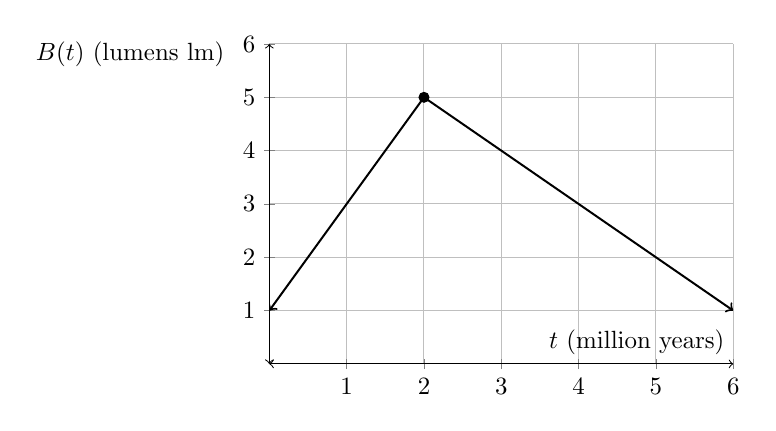
\begin{tikzpicture}[scale=0.9]
\begin{axis}[
    xlabel={$t$ (million years)},
    ylabel={$B(t)$ (lumens lm)},
    ylabel style={at={(axis description cs:-0.3,0.9)},anchor=south},
    xmin=0, xmax=6,
    ymin=0, ymax=6,
    grid=both,
    width=3.2in,
    height=2.4in,
    xtick={0,1,2,3,4,5,6},
    ytick={0,1,2,3,4,5,6}
]

% Rising phase
\addplot[thick, <-] coordinates {(0,1) (2,5)};

% Declining phase
\addplot[thick, ->] coordinates {(2,5) (6,1)};

% Peak point
\addplot[only marks, mark=*] coordinates {(2,5)};

\end{axis}
\end{tikzpicture}
\end{center}

\begin{enumerate}

\item Calculate $B'(5)$. In terms of the context above, what does it represent? What are its units?

\vspace{1.5cm}

\noindent  \hfill Units:  \underline{\hspace{2.5in}}

\vspace{4cm}

\item Calculate the following value. 
\[
\frac{B(4)-B(1)}{4-1}
\]
In terms of the context above, what does it
represent? What are its units?

\vspace{1.5cm}

\noindent \hfill Units: \underline{\hspace{2.5in}}

\vspace{4cm}


% ================= TABLE SECTION =================

% \begin{minipage}[t][3.2in][t]{\textwidth}

% \begin{enumerate}
\item List all $t$ values for which $B'(t)$ does not exist. Explain why.:
\vspace{0.5cm}

\noindent \hfill $t=$ \underline{\hspace{2in}}

\vspace{3cm}

% \item[ii.] Mark the boxes in the table below to indicate what can be said about the given quantities.

% \end{enumerate}

% \vspace{-0.1in}

% \begin{tabular}{m{3.2in} m{0.7in} m{0.7in} m{0.7in}}
%  & positive? & negative? & zero?\\[0.15in]

% $\bullet$ $\displaystyle\lim_{t\to 1}\frac{B(t)-B(1)}{t-1}$ is $\dotfill$ 
% & $\square$ & $\square$ & $\square$ \\[0.25in]

% $\bullet$ $\displaystyle\frac{B(5)-B(3)}{5-3}$ is $\dotfill$ 
% & $\square$ & $\square$ & $\square$ \\[0.25in]

% $\bullet$ $B'(4)$ is $\dotfill$ 
% & $\square$ & $\square$ & $\square$ \\

% \end{tabular}

% \end{minipage}
\end{enumerate}


%%%%%%%%%%%%%%%%%%%%%%%%%%%%%%%%%%%%%%%%%%%%%%%%%%%%%
%%%%%%%%%%% END PROBLEM D1 %%%%%%%%%%%%%%%%%%%%%%%%%%
%%%%%%%%%%%%%%%%%%%%%%%%%%%%%%%%%%%%%%%%%%%%%%%%%%%%%

\newpage
%%%%%%%%%%%%%%%%%%%%%%%%%%%%%%%%%%%%%%%%%%%%%%%%%%%%%
%%%%%%%%%%% BEGIN PROBLEM D2 %%%%%%%%%%%%%%%%%%%%%%%%
%%%%%%%%%%%%%%%%%%%%%%%%%%%%%%%%%%%%%%%%%%%%%%%%%%%%%

\item Find the derivative of the following expressions. 

A correct final answer receives full credit. Nevertheless, you are encouraged to write down the steps so that you will be able to receive partial credit if you final answer is not fully correct. There's no need to simplify your final answer

\begin{enumerate}
\item $f(x) = e^x\cdot\dfrac{x^2}{x^3 + 2}$

\vfill

\item $g(x) = \sqrt{4x^2+5}$

\vfill 
\end{enumerate}

%%%%%%%%%%%%%%%%%%%%%%%%%%%%%%%%%%%%%%%%%%%%%%%%%%%%%
%%%%%%%%%%% END PROBLEM D2 %%%%%%%%%%%%%%%%%%%%%%%%%%
%%%%%%%%%%%%%%%%%%%%%%%%%%%%%%%%%%%%%%%%%%%%%%%%%%%%%
\newpage
%%%%%%%%%%%%%%%%%%%%%%%%%%%%%%%%%%%%%%%%%%%%%%%%%%%%%
%%%%%%%%%%% BEGIN PROBLEM D3 %%%%%%%%%%%%%%%%%%%%%%%%
%%%%%%%%%%%%%%%%%%%%%%%%%%%%%%%%%%%%%%%%%%%%%%%%%%%%%

\item Write down the derivatives of the following functions. No work required. No need to simplify.

If you need to write down your work, please do so at the bottom half of this page, not in the answer space.

\begin{center}
        \begin{tabular}{l c r l c r}
            %
            $\displaystyle\frac{d}{dx}\left[ 5x^6 \right]$ & $=$ & \rule[-8pt]{1.5in}{0.4pt} &
            %
            \vspace{2in}
            $\displaystyle\frac{d}{dx}\left[ 2^x-\dfrac{1}{x^2} \right]$ & $=$ & \rule[-8pt]{1.5in}{0.4pt}\\[0.3in]
            %%%%%
            \vspace{2in}
            $\displaystyle\frac{d}{dx}\left[ \left(\dfrac{2}{9}\right)^3 \right]$ & $=$ & \rule[-8pt]{1.5in}{0.4pt} & 
            %%%%%
            $\displaystyle\frac{d}{dx}\left[ \sqrt[5]{x^2}-2e^x+\ln(x)\right]$ & $=$ & \rule[-8pt]{1.5in}{0.4pt}\\[0.3in]
            %%%%%
            $\displaystyle\frac{d}{dx}\left[ \log_2(x) \right]$ & $=$ & \rule[-8pt]{1.5in}{0.4pt}&
            %
            $\displaystyle\frac{d}{dx}\left[ \dfrac{-7x^4+3x^5-2x}{x^4} \right]$ & $=$ & \rule[-8pt]{1.5in}{0.4pt}\\[0.3in]
        \end{tabular} 
\end{center}

%%%%%%%%%%%%%%%%%%%%%%%%%%%%%%%%%%%%%%%%%%%%%%%%%%%%%
%%%%%%%%%%% END PROBLEM D3 %%%%%%%%%%%%%%%%%%%%%%%%%%
%%%%%%%%%%%%%%%%%%%%%%%%%%%%%%%%%%%%%%%%%%%%%%%%%%%%%


\newpage

%%%%%%%%%%%%%%%%%%%%%%%%%%%%%%%%%%%%%%%%%%%%%%%%%%%%%
%%%%%%%%%%% BEGIN PROBLEM I1 %%%%%%%%%%%%%%%%%%%%%%%%
%%%%%%%%%%%%%%%%%%%%%%%%%%%%%%%%%%%%%%%%%%%%%%%%%%%%%

\item The rate at which immune cells perform phagocytosis is $r(t)$ - the total number of pathogens eliminated by the immune system in thousand pathogens engulfed per hour, where $t$ is the number of hours after a bacterial infection enters the bloodstream.

Below is a graph of $r(t)$.

\begin{center}
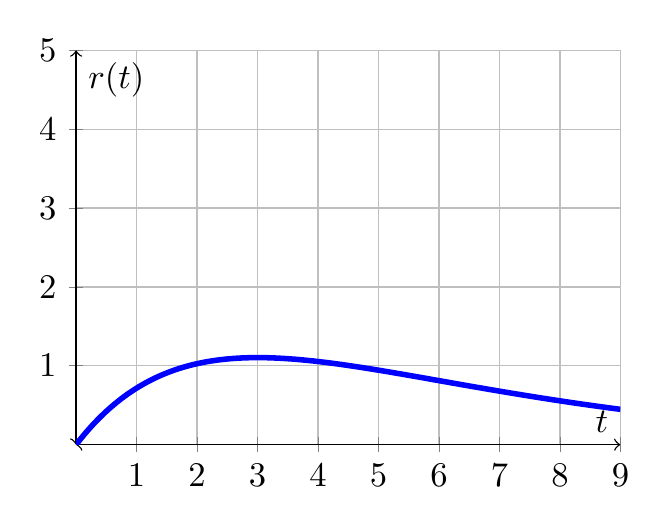
\begin{tikzpicture}[scale=1.25]
\begin{axis}[
    xlabel={$t$},
    ylabel={$r(t)$},
    xtick={1,2,3,4,5,6,7,8,9},
    ytick={0,1,2,3,4,5},
    xmin=0, xmax=9,
    ymin=0, ymax=5,
    grid=both,
    height=2.2in,
    width=2.8in
]

% smooth immune response curve (rise and fall)
\addplot[blue, ultra thick, domain=0:9, samples=200] {x*exp(-x/3)};

\end{axis}
\end{tikzpicture}
\end{center}
\begin{enumerate}


\item What is the meaning of
\[
\int_{3}^{5} r(t)\,dt = 2
\]
in this biological context? Make sure to include units in your explanation.

\vfill
\vfill

\item Is
\[
\int_{4}^{6} r(t)\,dt
\]
positive, negative, or zero? No justification required. \textbf{Note:} $r(t)$ is positive and decreasing from 4 hours to 6 hours after infection begins. Based on this, 

\vfill


\item Write an expression representing the total number of pathogens eliminated by the immune system during the first $9$ hours after a bacterial infection enters the bloodstream.

\vfill
\vfill

\end{enumerate}
%%%%%%%%%%%%%%%%%%%%%%%%%%%%%%%%%%%%%%%%%%%%%%%%%%%%%
%%%%%%%%%%% END PROBLEM I1 %%%%%%%%%%%%%%%%%%%%%%%%%%
%%%%%%%%%%%%%%%%%%%%%%%%%%%%%%%%%%%%%%%%%%%%%%%%%%%%%

\newpage

%%%%%%%%%%%%%%%%%%%%%%%%%%%%%%%%%%%%%%%%%%%%%%%%%%%%%
%%%%%%%%%%% BEGIN PROBLEM I3 %%%%%%%%%%%%%%%%%%%%%%%%
%%%%%%%%%%%%%%%%%%%%%%%%%%%%%%%%%%%%%%%%%%%%%%%%%%%%%

\item Write down the indefinite integrals of the following expressions. 

Although no work is required, you are encouraged to include any work that shows your thought process. 

%constant, power, exponential, log, +C, algebraic manipulation

\begin{center}
        \begin{tabular}{l c r l c r}
            %
            $\displaystyle\int 4x^2\,dx$ & $=$ & \rule[-8pt]{1.5in}{0.4pt} &
            %
            \vspace{2in}
            $\displaystyle\int \dfrac{2}{x^4} \,dx$ & $=$ & \rule[-8pt]{1.5in}{0.4pt}\\[1in]
            %%%%%
            $\displaystyle\int \dfrac{1}{x}+1\,dx$ & $=$ & \rule[-8pt]{1.5in}{0.4pt}&
            %
            \vspace{2in}
            $\displaystyle\int 3^x\,dx$ & $=$ & \rule[-8pt]{1.5in}{0.4pt}\\[1in]
            %%%%%
            $\displaystyle\int e^x-2x \,dx$ & $=$ & \rule[-8pt]{1.5in}{0.4pt} & 
            %
            $\displaystyle\int \sqrt[5]{x^4} \,dx$ & $=$ & \rule[-8pt]{1.5in}{0.4pt}\\[0.3in]
            %%%%%
        \end{tabular}
\end{center}

%%%%%%%%%%%%%%%%%%%%%%%%%%%%%%%%%%%%%%%%%%%%%%%%%%%%%
%%%%%%%%%%% END PROBLEM I3 %%%%%%%%%%%%%%%%%%%%%%%%%%
%%%%%%%%%%%%%%%%%%%%%%%%%%%%%%%%%%%%%%%%%%%%%%%%%%%%%

\newpage

%%%%%%%%%%%%%%%%%%%%%%%%%%%%%%%%%%%%%%%%%%%%%%%%%%%%%
%%%%%%%%%%% BEGIN PROBLEM I4 %%%%%%%%%%%%%%%%%%%%%%%%
%%%%%%%%%%%%%%%%%%%%%%%%%%%%%%%%%%%%%%%%%%%%%%%%%%%%%

\item For each of the following definite integrals, determine whether the Fundamental Theorem of Calculus (FTC) can be applied to evaluate. 

If so, evaluate the integral using the FTC. There's no need to simplify your final answer.

If not, clearly indicate that and explain why.

\begin{enumerate}
    \item $\displaystyle\int_{-1}^{1}\frac{1}{x^{2}}+4x^3-e^x\, dx$

    \vfill

    \item $\displaystyle\int_{-1}^1 3x^2+\frac{1}{\sqrt[3]{x}}-1\, dx$

    \vfill
\end{enumerate}

%%%%%%%%%%%%%%%%%%%%%%%%%%%%%%%%%%%%%%%%%%%%%%%%%%%%%
%%%%%%%%%%% END PROBLEM I4 %%%%%%%%%%%%%%%%%%%%%%%%%%
%%%%%%%%%%%%%%%%%%%%%%%%%%%%%%%%%%%%%%%%%%%%%%%%%%%%%

\newpage

%%%%%%%%%%%%%%%%%%%%%%%%%%%%%%%%%%%%%%%%%%%%%%%%%%%%%
%%%%%%%%%%% BEGIN PROBLEM F3 %%%%%%%%%%%%%%%%%%%%%%%%
%%%%%%%%%%%%%%%%%%%%%%%%%%%%%%%%%%%%%%%%%%%%%%%%%%%%%

\item \begin{enumerate}
    \item Find the value of the following expressions. \textbf{Show all work.} Simplify as much as possible so that your final answer is a number.

    \begin{enumerate}
        \item[(i)] $\displaystyle\sum_{i=3}^4\dfrac{i}{i-2}$

        \vfill

        \item[(ii)] $\displaystyle\sum_{j=2}^52$ 

        \vfill
    \end{enumerate}

    \item Rewrite the following in summation notation. 

    \[\ln(1)+2\ln(2)+4\ln(3)+8\ln(4)\]

    \vfill
\end{enumerate}

%%%%%%%%%%%%%%%%%%%%%%%%%%%%%%%%%%%%%%%%%%%%%%%%%%%%%
%%%%%%%%%%% END PROBLEM F3 %%%%%%%%%%%%%%%%%%%%%%%%%%
%%%%%%%%%%%%%%%%%%%%%%%%%%%%%%%%%%%%%%%%%%%%%%%%%%%%%

\newpage

%%%%%%%%%%%%%%%%%%%%%%%%%%%%%%%%%%%%%%%%%%%%%%%%%%%%%
%%%%%%%%%%% BEGIN PROBLEM L1 %%%%%%%%%%%%%%%%%%%%%%%%
%%%%%%%%%%%%%%%%%%%%%%%%%%%%%%%%%%%%%%%%%%%%%%%%%%%%%

\item \begin{enumerate}
    
    \item Write down the three continuity conditions:
    
    \
    
        \begin{itemize}
        \item[i.] \hrulefill\\[0.1in]
        \item[ii.] \hrulefill\\[0.1in]
        \item[iii.] \hrulefill\\
        \end{itemize}
\vspace{1cm}

\item For each graph below, identify the type of discontinuity at $x=1$ - removable, jump, infinite. If the graph is continuous, state so.


    \end{enumerate}

\vspace{0.4em}

\noindent
\begin{tabular}{ccc}

% ================= GRAPH 1 =================
\begin{minipage}{0.3\textwidth}
\centering
\textbf{A}
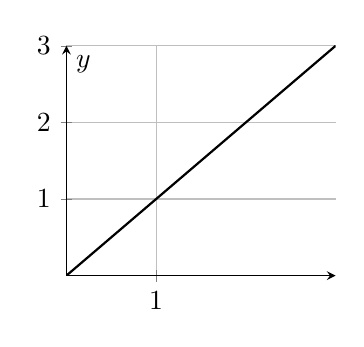
\begin{tikzpicture}
\begin{axis}[
    axis lines=middle,
    xmin=0, xmax=3,
    ymin=0, ymax=3,
    grid=both,
    width=5cm,
    height=4.5cm,
    xtick={1},
    ytick={1,2,3},
    xlabel={}
]
\addplot[thick, domain=0:3] {x};
\end{axis}
\end{tikzpicture}
\vspace{2cm}

Type:\hrulefill


\vspace{0.8cm}

\end{minipage}
&
% ================= GRAPH 2 =================
\begin{minipage}{0.3\textwidth}
\centering
\textbf{B}
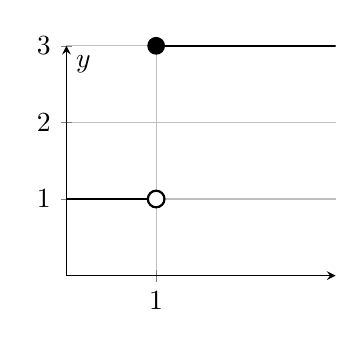
\begin{tikzpicture}
\begin{axis}[
    axis lines=middle,
    xmin=0, xmax=3,
    ymin=0, ymax=3,
    grid=both,
    width=5cm,
    height=4.5cm,
    xtick={1},
    xlabel={}
]

\addplot[thick, domain=0:1] {1};
\addplot[thick, domain=1:3] {3};

% Open circle (hole) at (1,1)
\addplot[
    only marks,
    mark=*,
    mark size=3pt,
    color=white
] coordinates {(1,1)};

\addplot[
    only marks,
    mark=o,
    mark size=3pt,
    thick,
    color=black
] coordinates {(1,1)};

% Filled black dot at (1,3)
\addplot[
    only marks,
    mark=*,
    mark size=3pt,
    color=black
] coordinates {(1,3)};
\end{axis}
\end{tikzpicture}
\vspace{2cm}

Type:\hrulefill


\vspace{0.8cm}

\end{minipage}
&
% ================= GRAPH 3 =================
\begin{minipage}{0.3\textwidth}
\centering
\textbf{C}
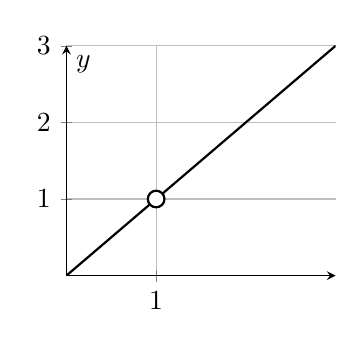
\begin{tikzpicture}
\begin{axis}[
    axis lines=middle,
    xmin=0, xmax=3,
    ymin=0, ymax=3,
    grid=both,
    width=5cm,
    height=4.5cm,
    xtick={1},
    xlabel={}
]

\addplot[thick, domain=0:3] {x};
\addplot[
    only marks,
    mark=*,
    mark size=3pt,
    color=white
] coordinates {(1,1)};
\addplot[only marks, mark=o,thick,mark size=3pt,
mark options={fill=white}]
coordinates {(1,1)};

\end{axis}
\end{tikzpicture}
\vspace{2cm}

Type:\hrulefill


\vspace{0.8cm}

\end{minipage}

\\
\end{tabular}
\vspace{1cm}

    \begin{enumerate}
    
    \item[(c)] For each of the three graphs above, which continuity conditions(s) are violated at $x=1$, if any? No justification required. Write down all violated conditions for each sketch to earn full credit.
    \vspace{2.5cm}
    
    \textbf{A}:\hrulefill \quad \textbf{B}:\hrulefill \quad \textbf{C}:\hrulefill

    \end{enumerate}

%%%%%%%%%%%%%%%%%%%%%%%%%%%%%%%%%%%%%%%%%%%%%%%%%%%%%
%%%%%%%%%%% END PROBLEM L1 %%%%%%%%%%%%%%%%%%%%%%%%%%
%%%%%%%%%%%%%%%%%%%%%%%%%%%%%%%%%%%%%%%%%%%%%%%%%%%%%

\newpage

%%%%%%%%%%%%%%%%%%%%%%%%%%%%%%%%%%%%%%%%%%%%%%%%%%%%%
%%%%%%%%%%% BEGIN PROBLEM P1 %%%%%%%%%%%%%%%%%%%%%%%%
%%%%%%%%%%%%%%%%%%%%%%%%%%%%%%%%%%%%%%%%%%%%%%%%%%%%%

\item In a simplified game of UNO, a player draws one card from a special deck.
\begin{itemize}
    \item There is a 10\% chance the card is a Wild Draw Four, which gives the player 4 points.
    \item There is a 20\% chance the card is a standard Wild Card, which gives the player 2 points.
    \item Otherwise, the card is a normal card, which gives the player 0 points.
\end{itemize}
Let $X$ be a discrete random variable representing the number of points a player earns from drawing one card.

\begin{enumerate}

\item What are the possible values of $X$?

\vfill

\item Write down the probability mass function $p(x)$ of $X$ using either a table or a list of values and probabilities.

\vfill
\vfill

\item Find the expected value of $X$.

\vfill
\vfill

\item Find the variance of $X$.

\vfill
\vfill

\end{enumerate}
%%%%%%%%%%%%%%%%%%%%%%%%%%%%%%%%%%%%%%%%%%%%%%%%%%%%%
%%%%%%%%%%% END PROBLEM P1 %%%%%%%%%%%%%%%%%%%%%%%%%%
%%%%%%%%%%%%%%%%%%%%%%%%%%%%%%%%%%%%%%%%%%%%%%%%%%%%%

\newpage

%%%%%%%%%%%%%%%%%%%%%%%%%%%%%%%%%%%%%%%%%%%%%%%%%%%%%
%%%%%%%%%%% BEGIN PROBLEM P2 %%%%%%%%%%%%%%%%%%%%%%%%
%%%%%%%%%%%%%%%%%%%%%%%%%%%%%%%%%%%%%%%%%%%%%%%%%%%%%

\item Let $X$ be a continuous random variable with the following probability density function.

\[p(x)=\begin{cases}2x\qquad 0\le x\le 1\\ 0 \qquad \text{otherwise}\end{cases}\]

\begin{enumerate}
    \item Find $P(0<X<\frac{1}{2})$.
    \vfill

    \item What is the support of $X$?

    \vfill

    \item Find the expectation $E[X]$ of $X$.

    \vfill
    
    % \item Find the variance 


    \vfill
\end{enumerate}

%%%%%%%%%%%%%%%%%%%%%%%%%%%%%%%%%%%%%%%%%%%%%%%%%%%%%
%%%%%%%%%%% END PROBLEM P2 %%%%%%%%%%%%%%%%%%%%%%%%%%
%%%%%%%%%%%%%%%%%%%%%%%%%%%%%%%%%%%%%%%%%%%%%%%%%%%%%

\end{enumerate}

\newpage

This page is left blank intentionally.\\

Use this page if you need additional space to write your solutions to any problem. \\

If you wish this page graded, you must refer to this page on \textbf{the original page} of the problem. Otherwise, your grader will NOT consider your work on this page.

\newpage

This page is left blank intentionally.\\

Use this page if you need additional space to write your solutions to any problem. \\

If you wish this page graded, you must refer to this page on \textbf{the original page} of the problem. Otherwise, your grader will NOT consider your work on this page.

\end{document}